%%%%%%%%%%%%%%%%%%%%%%%%%%%%%%%%%%%%%%%%%%%%%%%%%%%%%%%%%%%%
%%  This Beamer template was created by Cameron Bracken.
%%  Anyone can freely use or modify it for any purpose
%%  without attribution.
%%
%%  The current presentation created by Jeferson L. R. Souza (jefecomp) is based on the template created by Cameron Bracken. 
%%  
%%  Small modifications have been introduced and anyone is free to use such modified version.
%%
%% Last Modified: June 14, 2015.

\documentclass[xcolor=x11names,compress]{beamer}

%% General document %%%%%%%%%%%%%%%%%%%%%%%%%%%%%%%%%%
\usepackage{graphicx}
\usepackage{tikz}
\usetikzlibrary{decorations.fractals}
%%%%%%%%%%%%%%%%%%%%%%%%%%%%%%%%%%%%%%%%%%%%%%%%%%%%%%

%Hyperref
\usepackage{hyperref}

%Multirow package
\usepackage{multirow} 

%Math packages
\usepackage{amsmath}
\usepackage{textcomp}


%% Beamer Layout %%%%%%%%%%%%%%%%%%%%%%%%%%%%%%%%%%
\useoutertheme[footline=authorinstitutetitle,subsection=false,shadow]{miniframes}
\useinnertheme{default}
\usefonttheme{professionalfonts}
\usepackage{mathpazo}

\setbeamerfont{title like}{shape=\scshape,series=\bfseries}
\setbeamerfont{frametitle}{shape=\scshape,series=\bfseries}

\setbeamercolor*{lower separation line head}{bg=Green3} 
\setbeamercolor*{upper separation line foot}{bg=Green3} 
\setbeamercolor*{normal text}{fg=black,bg=white} 
\setbeamercolor*{alerted text}{fg=black,bg=black!10} 
\setbeamercolor*{example text}{fg=black} 
\setbeamercolor*{structure}{fg=black}
 
\setbeamercolor*{palette tertiary}{fg=black,bg=black!3} 
\setbeamercolor*{palette quaternary}{fg=black,bg=black!10} 

%%%%%%%%%%%%%%%%%%%%%%%%%%%%%%%%%%%%%%%%%%%%%%%%%%

\setbeamertemplate{blocks}[rounded] [shadow=true]
\setbeamertemplate{frametitle continuation}[from second][(Continuação)]

%%  declaring picture extensions and default path
\DeclareGraphicsExtensions{.png, .jpg, .pdf}
\graphicspath{{pictures/}}

%% Supporting source code lists
\usepackage{listings}
\lstset{breakatwhitespace,
language=Java,
columns=fullflexible,
keepspaces,
breaklines,
tabsize=3, 
showstringspaces=false,
extendedchars=true}

%Text position
\usepackage{textpos}
\setlength{\TPHorizModule}{128mm}
\setlength{\TPVertModule}{96mm}

\usepackage{array}

%Puting text and other float elements over pictures
\usepackage[percent]{overpic}


%% Hyperlinks over all the document
\usepackage{hyperref}

%% Controlling text alignment
\usepackage{ragged2e}

%% Framed text
\usepackage{framed}

%% Math packages
\usepackage{amsmath}

\begin{document}

\title[Linguagem de Definição de Dados (DDL) \hskip13mm \insertframenumber / \inserttotalframenumber  \hskip33.5mm \inserttitlegraphic]{Linguagem de Definição de Dados (DDL) \\[4mm]

\includegraphics[keepaspectratio,width=.25\textwidth]{database-server}}
\author[@2018 Prof. Jeferson Souza, MSc (jefecomp) - All rights reserved.]{
	\textcolor{blue}{Prof. Jeferson Souza, MSc.} \\[1mm] 
	\textcolor{blue}{\textit{{\footnotesize (jefecomp) }}}\\[1.5mm]
	 \underline{{\footnotesize jeferson.souza@udesc.br}}
	 \vspace*{1mm}
}
\institute[]{\centering 
\includegraphics[keepaspectratio,width=.5\textwidth]{template/logo_udesc_joinville_horizontal_assinatura}
}

\date{}

\titlegraphic{
\includegraphics[keepaspectratio,width=.2\textwidth]{template/logo_udesc_joinville_horizontal_assinatura}}

%%%%%%%%%%%%%%%%%%%%%%%%%%%%%%%%%%%%%%%%%%%%%%%%%%%%%%
%%%%%%%%%%%%%%%%%%%%%%%%%%%%%%%%%%%%%%%%%%%%%%%%%%%%%%
\begin{frame}[plain,noframenumbering]
\titlepage
\end{frame}


%%%%%%%%%%%%%%%%%%%%%%%%%%%%%%%%%%%%%%%%%%%%%%%%%%%%%%
%%%%%%%%%%%%%%%%%%%%%%%%%%%%%%%%%%%%%%%%%%%%%%%%%%%%%%
\section{Anteriormente}
\subsection{Representação Schemas}

\begin{frame}{Representação Gráfica e Simplificada do Schema}

\begin{itemize}
\itemsep 5mm

\item Nas aulas anteriores vimos uma representação usando tabelas e comparamos com a representação realizada através do diagrama E-R;

\item Agora veremos uma forma que permite uma visão ``simplificada" dessas duas representações: O \underline{diagrama de esquema}.

\end{itemize}

\end{frame}

\begin{frame}{Diagrama de Schema}

\centering 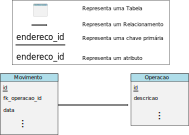
\includegraphics[keepaspectratio, width=.8\textwidth]{schema_diagram}


\end{frame}

%%%%%%%%%%%%%%%%%%%%%%%%%%%%%%%%%%%%%%%%%%%%%%%%%%%%%%
%%%%%%%%%%%%%%%%%%%%%%%%%%%%%%%%%%%%%%%%%%%%%%%%%%%%%%
\section{Introdução à DDL}
\subsection{Introdução à DDL}
\begin{frame}{Introdução à Linguagem de Definição de Dados (DDL)}

\begin{itemize}
\itemsep 5mm

\item Subconjunto da linguagem SQL;

\item A sigla DDL é derivada do inglês Data Definition Language;

\item Permite a criação de toda a estrutura de dados (dentro de um schema), incluindo tabelas, relacionamento, restrições, visões, entre outros.

\item Permite especificar restrições sobre a estrutura de dados criada no banco. Exemplo: coluna nome na tabela ``Usuario" não pode ser nulo.

\end{itemize}

\end{frame}

\begin{frame}[allowframebreaks=.7]{Tipos de Restrições}

\begin{itemize}
\itemsep 5mm

\item Domínio: assegura que os valores de uma dada coluna estão dentro de um domínio esperado;

\item Integridade referencial: assegura que informações de uma dada coluna que fazem referências a dados de outra tabela existem, e são consistentes;

\item Asserções: restrições que devem ser satisfeitas pela base de dados. Ex: Toda conta bancária deve ter, obrigatoriamente, um titular associado. Restrições de \underline{domínio} e \underline{integridade referencial} são casos especiais das asserções;

\item Autorização: autoriza ou não autoriza o acesso aos dados a usuários da base de dados. Restrições mais comuns: leitura, inserção, atualização, remoção. 

\end{itemize}
\end{frame}

%%%%%%%%%%%%%%%%%%%%%%%%%%%%%%%%%%%%%%%%%%%%%%%%%%%%%%
%%%%%%%%%%%%%%%%%%%%%%%%%%%%%%%%%%%%%%%%%%%%%%%%%%%%%%
\section{Base de Dados}
\subsection{Base de Dados}

\begin{frame}{Criar Bases de Dados}

\centering 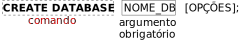
\includegraphics[keepaspectratio,width=\textwidth]{create_database}

\begin{block}{}
As opções incluem desde da especificação do ``dono" da base de dados, até a indicação de qual template utilizar para criar a base de dados.
\end{block}

\pause 

\begin{alertblock}{\centering Dica}
Consultem a ajuda ({\textbackslash}h) do psql para ver detalhes do comando, já que vamos utilizar o PostgreSQL durante o curso.
\end{alertblock}


\end{frame}

\begin{frame}{Criar Bases de Dados}

\begin{alertblock}{Exemplo}
\centering \textbf{CREATE DATABASE} banii;
\end{alertblock}

\pause

\begin{alertblock}{\centering \textcolor{red}{Detalhe Importante}}
Não esqueçam de terminar os comandos com ponto e vírgula (;).
\end{alertblock}

\end{frame}

\begin{frame}{Criar Base de Dados Modelo}

\begin{alertblock}{Exemplo}
\centering \textbf{CREATE DATABASE} banii \textbf{IS\_TEMPLATE}=true;
\end{alertblock}

\end{frame}

\begin{frame}{Criar Bases de Dados com Modelo Específico}

\begin{alertblock}{Exemplo}
\centering \textbf{CREATE DATABASE} banii\_rocks \textbf{WITH TEMPLATE}=banii;
\end{alertblock}

\end{frame}

\begin{frame}{Remover Base de Dados}

\centering 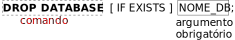
\includegraphics[keepaspectratio,width=\textwidth]{drop_database}

\end{frame}

\begin{frame}{Remover Base de Dados}

\begin{alertblock}{Exemplo 1}
\centering \textbf{DROP DATABASE} banii;
\end{alertblock}

\pause

\begin{alertblock}{Exemplo 2}
\centering \textbf{DROP DATABASE IF EXISTS} banii;
\end{alertblock}

\pause

\begin{alertblock}{\textbf{DROP DATABASE} VS \textbf{DROP DATABASE IF EXISTS}}
Sem a utilização do \textbf{IF EXISTS} ao tentar remover uma base de dados que não existe, um erro será apresentado. Com o \textbf{IF EXISTS}, caso a base de dados não exista, o comando termina sem erros.
\end{alertblock}

\end{frame}

%%%%%%%%%%%%%%%%%%%%%%%%%%%%%%%%%%%%%%%%%%%%%%%%%%%%%%
%%%%%%%%%%%%%%%%%%%%%%%%%%%%%%%%%%%%%%%%%%%%%%%%%%%%%%
\section{Schema}
\subsection{Schema}

\begin{frame}{Criar Schema}

\centering 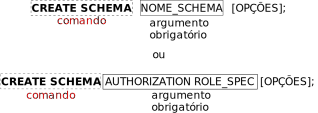
\includegraphics[keepaspectratio,width=\textwidth]{create_schema}

\pause

\begin{block}{}
\centering Existe mais duas variações que veremos durante as aulas práticas que usam a cláusula \textbf{IF NOT EXISTS}.
\end{block}

\end{frame}

\begin{frame}{Criar Schema}

\begin{alertblock}{Exemplo 1}
\textbf{CREATE SCHEMA} banii\_schema;
\end{alertblock}

\begin{alertblock}{Exemplo 2}
\textbf{CREATE SCHEMA} AUTHORIZATION postgres;
\end{alertblock}

\pause 

\begin{alertblock}{\centering \textcolor{red}{Importante!}}
No Exemplo 2 o nome do schema criado é o mesmo do nome do usuário, ou seja, \underline{postgres}.
\end{alertblock}

\end{frame}

\begin{frame}{Remover Schema}

\centering 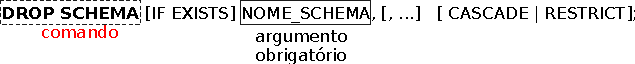
\includegraphics[keepaspectratio,width=\textwidth]{drop_schema}

\pause 

\begin{alertblock}{\centering \textcolor{red}{Importante!}}
RESTRICT é o comportamento padrão do comando, ou seja, não é possível remover um schema que não esteja vazio;
\end{alertblock}

\end{frame}

\begin{frame}{Remover Schema}

\begin{alertblock}{Exemplo 1}
\centering \textbf{DROP SCHEMA} banii\_schema;
\end{alertblock}

\begin{alertblock}{Exemplo 2}
\centering \textbf{DROP SCHEMA} banii\_schema CASCADE;
\end{alertblock}

\pause

\begin{alertblock}{\centering Nota}
O parâmetro CASCADE indica que todo conteúdo do schema também será removido.
\end{alertblock}

\end{frame}

%%%%%%%%%%%%%%%%%%%%%%%%%%%%%%%%%%%%%%%%%%%%%%%%%%%%%%
%%%%%%%%%%%%%%%%%%%%%%%%%%%%%%%%%%%%%%%%%%%%%%%%%%%%%%
\section{Tipos de dados}
\subsection{Tipos de Dados}

\begin{frame}[allowframebreaks]{Tipos de Dados}

Os tipos básicos de dados são (\cite{SilberchatzEtAl2011}):

\begin{itemize}
\itemsep 5mm

\item char(n): tipo de tamanho fixo para armazenar, no máximo, n caracteres; 

\item varchar(n): tipo de tamanho variável para armazenar, no máximo, n caracteres.

\item int: tipo para armazenar valores inteiros. Tamanho depende da arquitetura do computador;

\item smallint: tipo para armazenar valores inteiros de menor tamanho. Tamanho depende da  arquitetura do computador;

\item numeric(p,d): tipo numérico para armazenar valores com precisão definida pelo usuário. O argumento \underline{p} indica o número de digitos inteiros (mais o sinal), e o argumento \underline{d} o número de digitos da parte não inteira (depois da vírgula); 

\item real, double precision: tipo para representar números de ponto flutuante com precisão dependente da arquitetura do computador;

\item float(n): tipo para armazenar números de ponto flutuante com precisão de n dígitos.

\end{itemize}

\begin{alertblock}{\centering Nota}
É importante consultar o manual do banco de dados para verificar as declarações de tipos específicos. No nosso caso, consultem o manual do PostgreSQL. \\[5mm] \underline{Não esqueçam}: O manual é o vosso melhor amigo (Além do professor, é claro :-D). 
\end{alertblock}

\end{frame}

%%%%%%%%%%%%%%%%%%%%%%%%%%%%%%%%%%%%%%%%%%%%%%%%%%%%%%
%%%%%%%%%%%%%%%%%%%%%%%%%%%%%%%%%%%%%%%%%%%%%%%%%%%%%%
\section{Tabelas}
\subsection{Criação de Tabelas}

\begin{frame}{Criar Tabela}

\centering 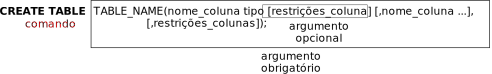
\includegraphics[keepaspectratio,width=\textwidth]{create_table}

\end{frame}

\begin{frame}{Criar Tabela}

\begin{alertblock}{Exemplo 1}

\textbf{CREATE TABLE} usuario(id \textcolor{red}{bigint}, nome \textcolor{red}{varchar}(20), email \textcolor{red}{varchar}(30));

\end{alertblock}

\begin{alertblock}{Exemplo 2}

\textbf{CREATE TABLE} banii\_schema.usuario(id \textcolor{red}{bigint}, nome \textcolor{red}{varchar}(20), email \textcolor{red}{varchar}(30));

\end{alertblock}

\pause 

\begin{alertblock}{\centering Pergunta:}

As tabelas criadas nos exemplos acima evitam a inserção de dados com todas as colunas iguais (i.e. dados repetidos)?

\end{alertblock}

\end{frame}

\begin{frame}{Criar Tabela com Chave Primária}

\begin{alertblock}{Exemplo 1}

\textbf{CREATE TABLE} usuario(id \textcolor{red}{bigint} \textit{PRIMARY KEY}, nome \textcolor{red}{varchar}(20), email \textcolor{red}{varchar}(30));

\end{alertblock}

\begin{alertblock}{Exemplo 2}

\textbf{CREATE TABLE} usuario(id \textcolor{red}{bigint}, nome \textcolor{red}{varchar}(20), email \textcolor{red}{varchar}(30), \textit{PRIMARY KEY}(id));

\end{alertblock}

\end{frame}

\begin{frame}[allowframebreaks]{Criar Tabela com Valores Incrementados Automaticamente}

Para criar tabelas com valores incrementados automaticamente no PostgreSQL basta utilizar um dos tipos serial.

\begin{alertblock}{Exemplo 1}

\textbf{CREATE TABLE} usuario(id \textcolor{red}{bigserial} \textit{PRIMARY KEY}, nome \textcolor{red}{varchar}(20), email \textcolor{red}{varchar}(30));

\end{alertblock}

\begin{alertblock}{Exemplo 2}

\textbf{CREATE TABLE} usuario(id \textcolor{red}{serial}, nome \textcolor{red}{varchar}(20), email \textcolor{red}{varchar}(30),\textit{PRIMARY KEY}(id));

\end{alertblock}

\begin{alertblock}{\centering Nota}
\centering Existe outra forma de criar tabelas com valores incrementados automaticamente, como veremos mais a frente no curso.
\end{alertblock}

\end{frame}


\begin{frame}[allowframebreaks]{Criar Tabela com Chave Estrangeira}

\begin{alertblock}{Exemplo 1}
\textbf{CREATE TABLE} endereco(id \textcolor{red}{bigserial} \textit{PRIMARY KEY}, logradouro \textcolor{red}{varchar}(50), cep \textcolor{red}{char}(8), cidade\_id \textcolor{red}{bigint} references cidade);
\end{alertblock}

\begin{alertblock}{Exemplo 2}
\textbf{CREATE TABLE} endereco(id \textcolor{red}{bigserial} \textit{PRIMARY KEY}, logradouro \textcolor{red}{varchar}(50), cep \textcolor{red}{char}(8), cidade\_id \textcolor{red}{bigint} references cidade(id));
\end{alertblock}

\begin{alertblock}{Exemplo 3}
\textbf{CREATE TABLE} endereco(id \textcolor{red}{bigserial} \textit{PRIMARY KEY}, logradouro \textcolor{red}{varchar}(50), cep \textcolor{red}{char}(8), cidade\_id \textcolor{red}{bigint}, \textit{FOREIGN KEY} (cidade\_id) references cidade(id));
\end{alertblock}

\end{frame}

\begin{frame}{Criar Tabela com Restrições nas Colunas}

Restrições mais comuns:

\begin{itemize}
\itemsep 5mm

\item NULL: coluna pode ou não conter valor (default);

\item NOT NULL: coluna deve SEMPRE conter valor;

\item UNIQUE: valor da couna deve ser único;

\item DEFAULT: especifica um valor default para uma coluna.

\end{itemize}

\end{frame}

\begin{frame}[allowframebreaks]{Criar Tabela com Restrições nas Colunas}

\begin{alertblock}{Exemplo 1}
\textbf{CREATE TABLE} endereco(id \textcolor{red}{bigserial} \textit{PRIMARY KEY}, logradouro \textcolor{red}{varchar}(50), cep \textcolor{red}{char}(8) \textit{UNIQUE}, cidade\_id \textcolor{red}{bigint} references cidade);
\end{alertblock}

\begin{alertblock}{Exemplo 2}
\textbf{CREATE TABLE} endereco(id \textcolor{red}{bigserial} \textit{PRIMARY KEY}, logradouro \textcolor{red}{varchar}(50) \textit{DEFAULT} 'SEM RUA' , cep \textcolor{red}{char}(8), cidade\_id \textcolor{red}{bigint} references cidade(id));
\end{alertblock}

\begin{alertblock}{Exemplo 3}
\textbf{CREATE TABLE} endereco(id \textcolor{red}{bigserial} \textit{PRIMARY KEY}, logradouro \textcolor{red}{varchar}(50), cep \textcolor{red}{char}(8), cidade\_id \textcolor{red}{bigint} \textit{NOT NULL}, \textit{FOREIGN KEY} (cidade\_id) references cidade(id));
\end{alertblock}

\end{frame}

\subsection{Alteração de Tabelas}

\begin{frame}{Alterar Estrutura de Tabelas}

\centering 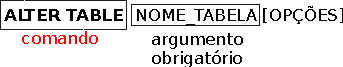
\includegraphics[keepaspectratio,width=\textwidth]{alter_table}

\begin{block}{}
As opções são muitas, e portanto serão apresentados alguns exemplos a seguir.
\end{block}

\end{frame}

\begin{frame}{Adicionar coluna a Tabela}

\begin{alertblock}{Exemplo 1}
\textbf{ALTER TABLE} endereco \textit{ADD} descricao \textcolor{red}{varchar}(30);
\end{alertblock}

\begin{alertblock}{Exemplo 2}
\textbf{ALTER TABLE} endereco \textit{ADD} estado\_id \textcolor{red}{bigint} references estado;
\end{alertblock}

\end{frame}

\begin{frame}{Remover coluna da Tabela}

\begin{alertblock}{Exemplo 1}
\textbf{ALTER TABLE} endereco \textit{DROP} descricao;
\end{alertblock}

\begin{alertblock}{Exemplo 2}
\textbf{ALTER TABLE} endereco \textit{DROP} descricao \textit{CASCADE};
\end{alertblock}

\end{frame}

\begin{frame}{Alterar Restrições de Coluna}

\begin{alertblock}{Exemplo }
\textbf{ALTER TABLE} endereco \textit{ALTER} descricao \textit{SET NOT NULL};
\end{alertblock}

\end{frame}

\begin{frame}{Adicionar Restrições a Coluna}

\begin{alertblock}{Exemplo 1}
\textbf{ALTER TABLE} endereco \textit{ADD} \textit{UNIQUE}(descricao);
\end{alertblock}

\begin{alertblock}{Exemplo 2}
\textbf{ALTER TABLE} endereco \textit{ADD} CONSTRAINT descricao\_unique \textit{UNIQUE}(descricao);
\end{alertblock}

\end{frame}

\begin{frame}{Remover Restrições da Coluna}

\begin{alertblock}{Exemplo}
\textbf{ALTER TABLE} endereco \textit{DROP} CONSTRAINT descricao\_unique;
\end{alertblock}

\begin{alertblock}{\textcolor{red}{Importante}}
É necessário saber o nome da restrição para remover a mesma da tabela.
\end{alertblock}

\end{frame}

\subsection{Remoção de Tabela}

\begin{frame}{Remover Tabela}

\centering 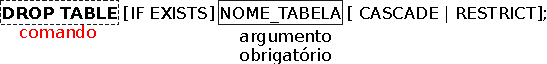
\includegraphics[keepaspectratio,width=\textwidth]{drop_table}

\end{frame}

\begin{frame}{Remover Tabela}

\begin{alertblock}{Exemplo 1}
\textbf{DROP TABLE} endereco;
\end{alertblock}

\begin{alertblock}{Exemplo 2}
\textbf{DROP TABLE} endereco CASCADE;
\end{alertblock}

\end{frame}

%%%%%%%%%%%%%%%%%%%%%%%%%%%%%%%%%%%%%%%%%%%%%%%%%%%%%%
%%%%%%%%%%%%%%%%%%%%%%%%%%%%%%%%%%%%%%%%%%%%%%%%%%%%%%
\section{}

\begin{frame}[plain,allowframebreaks,noframenumbering]{Bibliografia}

\begin{thebibliography}{Garcia-MolinaEtAl, 2008}

\bibitem[Garcia-MolinaEtAl, 2008]{Garcia-MolinaEtAl2008}

Garcia-Molina, H. and Ullman, J. D. and Widom, J.

\newblock{{\em ``Database Systems: The Complete Book"}. 2nd edition. Prentice Hall, 2008.}

\bibitem[PostgreSQLManual, 2018]{PostgreSQL10_2}

PostgreSQL Development Group.

\newblock{{\em ``PostgreSQL 10.2 Documentation"}. 2018.}

\bibitem[SilberchatzEtAl, 2011]{SilberchatzEtAl2011}

Silberschatz, A. and Korth, H.F. and Sudarshan, S.

\newblock	{{\em ``Database Systems"}. 6th edition. McGrawHill, 2011.}

\end{thebibliography}

\end{frame}

\begin{frame}[plain,noframenumbering]

\begin{center}

\includegraphics[keepaspectratio, width=.8\textwidth]{template/happycat-end}
\end{center}
\end{frame}

\end{document}